\documentclass[10pt,twocolumn,letterpaper]{article}

\usepackage{cvpr}
\usepackage{times}
\usepackage{epsfig}
\usepackage{graphicx}
\usepackage{amsmath}
\usepackage{amssymb}

\usepackage{cite}
\usepackage{wrapfig}
\usepackage{multirow}
\usepackage{caption}
\usepackage{subcaption}
\usepackage{verbatim}
\usepackage{booktabs}
\usepackage[ruled,vlined,linesnumbered]{algorithm2e}

% If you comment hyperref and then uncomment it, you should delete
% egpaper.aux before re-running latex.  (Or just hit 'q' on the first latex
% run, let it finish, and you should be clear).
\usepackage[pagebackref=true,breaklinks=true,letterpaper=true,colorlinks,bookmarks=false]{hyperref}

\cvprfinalcopy % *** Uncomment this line for the final submission

\def\cvprPaperID{****} % *** Enter the CVPR Paper ID here
\def\httilde{\mbox{\tt\raisebox{-.5ex}{\symbol{126}}}}

% Pages are numbered in submission mode, and unnumbered in camera-ready
\ifcvprfinal\pagestyle{empty}\fi
\begin{document}

%%%%%%%%% TITLE
\title{Image Colorization via Conditional Generative Adversarial Network}

\author{Luan Tran\\
Michigan State University\\
{\tt\small tranluan@msu.edu}
% For a paper whose authors are all at the same institution,
% omit the following lines up until the closing ``}''.
% Additional authors and addresses can be added with ``\and'',
% just like the second author.
% To save space, use either the email address or home page, not both
\and
Saif M. Imran\\
Michigan State University\\
{\tt\small imransai@msu.edu}
}

\maketitle
%\thispagestyle{empty}

%%%%%%%%% ABSTRACT
\begin{abstract}
We aim to color gray-scale images automatically, without direct human assistance.
This automatic colorization is an underconstrained problem
since there is usually no one-to-one correspondence between color and local texture.
In this work, we will try to apply recent advances in generative models which is Generative Adversarial Network~\cite{goodfellow2014generative} (GAN) to a conditional setting. Instead of generate realistic samples from random noise as conventional GAN, we will generate realistic samples (color image) from both input gray-scale image and noise.
\end{abstract}

%%%%%%%%% BODY TEXT
\section{Introduction}

Automated colorization of gray-scale images has been subject to much research within the computer vision and machine learning communities. Its capability has broad practical applications ranging from image enhancement to video restoration.

At first glance, hallucinating image colors seems impossible, since so much of the information (two out of the
three dimensions) has been lost. However, the semantics of the scene and its surface texture provide sufficient clues for many regions in each image (i.e the sea should be blue or the grass should be green). For this work, our goal is not necessarily to recover the actual ground truth color, but rather to produce a plausible colorization that could potentially fool a human observer. Therefore, our task becomes much more achievable: to model enough of the statistical dependencies between the semantics, the textures of gray-scale images and their color versions in order to produce visually compelling results.

%------------------------------------------------------------------------
\section{Proposed approach}
\begin{figure} [t!]
    \centering
    \begin{subfigure}[b]{0.48\textwidth}
        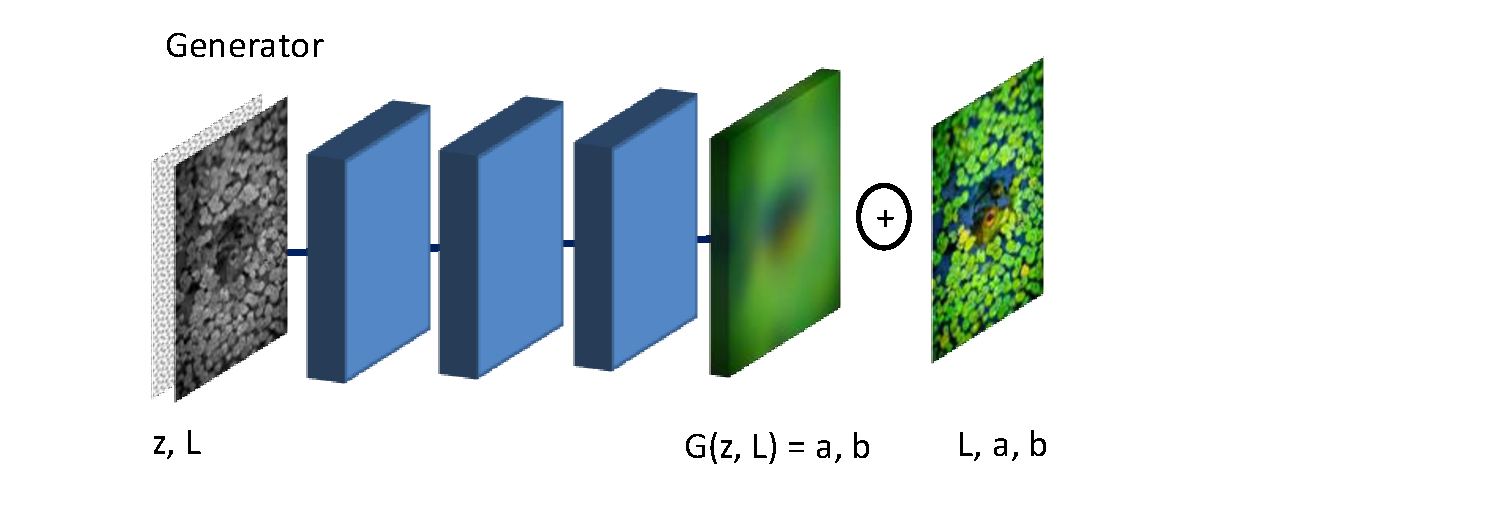
\includegraphics[trim=30 20 150 0, clip,width=\textwidth]{img/Generator.pdf}
    \end{subfigure}
    \begin{subfigure}[b]{0.48\textwidth}
        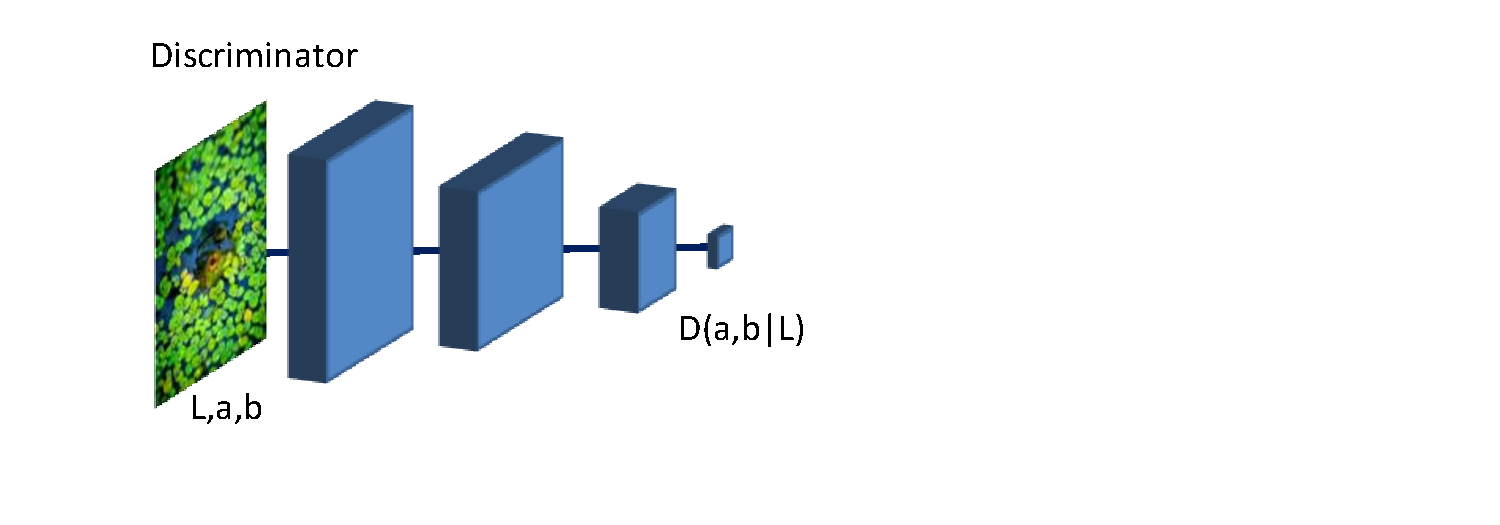
\includegraphics[trim=30 20 150 0, clip,width=\textwidth]{img/Discriminator.pdf}
    \end{subfigure}
    \vspace{-0.16in}
    \caption{\small Network architecture.}
    \vspace{-0.2in}
   \label{fig:concept}
\end{figure}


\subsection{Generative Adversarial Network} 

Our work is developed upon a recent trend in generative network, Generative Adversarial Network (GAN). GAN consists of a generator $G$ and a discriminator $D$ that compete in a two-player
minimax game: $D$ tries to distinguish between a real image $\bf{x}$ (come from data distribution $p_{data}(\mathbf{x})$) and a synthetic image $G(\bf{z})$; and $G$ tries to fool $D$ by synthesizing realistic-looking images. 
Concretely, $D$ and $G$ play the game with a value function $V(D,G)$:
\vspace{-1mm}
\begin{align}
\min_{G} \max_{D} V(D,G) =  E_{\mathbf{x} \sim p_{data}(\mathbf{x})} [\log D(\mathbf{x})] \nonumber \\ 
+  E_{\mathbf{z} \sim p_{z}(\mathbf{z})} [\log(1- D(G(\mathbf{z}))) ].
\end{align}
Goodfellow et al.~\cite{goodfellow2014generative} prove that this minimax game has
a global optimum when the distribution of the synthetic samples $p_{g}$, and that of the training samples $p_{data}$ are the same. 
Under mild conditions (e.g., $G$ and $D$ have enough capacity), $p_{g}$ converges to $p_{data}$. 
However, at the beginning of training, the samples generated from $G$ are extremely poor and are rejected by $D$ with high confidences. 
In practice, it is better for $G$ to maximize $\log(D(G(\mathbf{z})))$ instead of minimizing $\log \left( 1 - D(G(\mathbf{z})) \right)$~\cite{goodfellow2014generative}. 
As a result, $G$ and $D$ are trained to optimize the following functions:
\begin{align}
\max_{D} V_D(D,G) = {} & E_{\mathbf{x} \sim p_{data}(\mathbf{x})} [\log D({\bf{x}})] \nonumber \\ 
+ & E_{\mathbf{z} \sim p_{z}(\mathbf{z})} [\log(1- D(G(\mathbf{z}))) ], \\
\max_{G} V_G(D,G) = {} & E_{\mathbf{z} \sim p_{z}(\mathbf{z})} [\log(D(G(\mathbf{z})) ].
\end{align}

\subsection{Conditional Generative Adversarial Network} 
Gauthier~\cite{gauthier2014conditional} introduces an extension of GAN, which is conditional GAN, by adding a condition $\mathbf{y}$ to both $G$ and $D$. G accepts both noise data $\mathbf{z}$ along with an embedding $\mathbf{y}$ and produces an image $\mathbf{x}$. Meanwhile $D$ accepts an image $\mathbf{x}$ and condition $\mathbf{y}$ and predicts the probability under condition $\mathbf{y}$ that $\mathbf{x}$ came from the empirical data distribution rather than from the generative model.

The objective function for conditional GAN can be written as:
\begin{align}
 \min_{G} \max_{D} V(G,D) = E_{\mathbf{x} \sim p_{data}(\mathbf{x} | \mathbf{y})} [\log(D(\mathbf{x}|\mathbf{y}))] \nonumber \\
+  E_{z \sim p(z), \mathbf{y} \sim p_{data}(\mathbf{y}) } [\log(1-D(G(\mathbf{z,y}),\mathbf{y}))]
\end{align}

\subsection{Colorization GAN}

Our model is a direct application of conditional GAN. Each color image can be presented in Lab space. Any gray-scale input image can be treat as lightness component (L) of the final color out. Thus, we only need to estimate a, b component. The system consist of two network: generator ($G$) and discriminator ($D$). The generator take the gray-scale image ($L$) and random noise ($z$) as inputs and try to produce $a, b$ component of the image. Meanwhile D take all three components of images as inputs and try to distinguish between samples from the training data and generated samples. In other word, $D$ will produce one single value $D(a,b|L)$ that is probability $a, b$ is the true color component correspond to $L$. Both network $G, D$ will be train to optimize this function:
\begin{align}
 \min_{G} \max_{D} V(G,D) =  E_{a, b \sim p_{data}(a,b | L)} [\log(D(a,b|L))] \nonumber \\
                          + E_{z \sim p(z), L \sim p_{data}(L) } [\log(1-D(G(z,L),L))]
\end{align}




\section{Implementation Details}



\begin{table*}[t!]
\caption{\small Network architecture.}
\label{tab:network}
\begin{center}
\small
%\resizebox{0.7\linewidth}{!}{
\begin{tabular}{ @{}ccccccccccccc@{} }
\toprule
\multicolumn{3}{c}{$G$} & \hspace{2mm} 
& \multicolumn{3}{c}{$D$} \\
\cmidrule(r){1-3}
\cmidrule(r){5-7}

Layer & Filter Size & Output Size && Layer & Filter Size & Output Size \\ \midrule
Input  &       & $64\times64\times1$  && Input  &       & $64\times64\times3$ \\ \midrule
Conv11 & 3x3/1 & $64\times64\times32$ && Conv11& 3x3/1 & $64\times64\times32$ \\
Conv12 & 3x3/1 & $64\times64\times32$ && Conv12& 3x3/2 & $32\times32\times64$ \\ \midrule

Conv21 & 3x3/1 & $64\times64\times32$ && Conv21& 3x3/1 & $32\times32\times64$ \\
Conv22 & 3x3/1 & $64\times64\times32$ && Conv22& 3x3/2 & $16\times16\times128$ \\ \midrule

Conv31 & 3x3/1 & $64\times64\times32$ && Conv31& 3x3/1 & $16\times16\times128$ \\
Conv32 & 3x3/1 & $64\times64\times32$ && Conv32& 3x3/2 & $8\times8\times256$ \\   \midrule

Conv41 & 3x3/1 & $64\times64\times32$ && Conv41& 3x3/1 & $8\times8\times256$ \\
Conv42 & 3x3/1 & $64\times64\times32$ && Conv42& 3x3/2 & $4\times4\times256$ \\  \midrule

Conv5  & 3x3/1 & $64\times64\times2$  && FC     &       & $1$ \\ \bottomrule
\end{tabular}%}
\end{center}
\end{table*}

Our implementation is extensively modified from a publicly available implementation of DC-GAN~\footnote{https://github.com/carpedm20/DCGAN-tensorflow} using TensorFlow. In order to deal with any input size, $G$ will be a fully convolutional network as inspired by~\cite{long2015fully}. All convolution filter has size $3 \times 3$ as it has been shown to be effective in lasted CNN. 

Following the optimization strategy in~\cite{radford2015unsupervised}, all models are trained with a batch size of $64$. 
%using mini-batch SGD
All weights are initialized from a zero-centered normal distribution with a standard deviation of $0.02$. 
Adam optimizer~\cite{kingma2014adam} is used with a learning rate of $0.0002$ and momentum $0.5$.
%$\beta_1 = 0.5$.

In conventional GANs, Goodfellow et al.~\cite{goodfellow2014generative} suggest to alternate between $k$ (usually $k$ = 1) steps of optimizing $D$ and one step of optimizing $G$. 
This helps $D$ to maintain near-optimal solution as long as $G$ changes slowly. 


Our networks will be train and test on ImageNet dataset. To simplify the setup for $D$, all the training samples will have fixed size of $64\times 64$, which are randomly sample from origianl images in ImageNet. In the test state, sample images with any size can be used since it only go though the generator $G$. There is no pre-processing applied to the images except normalization to range $[-1,1]$. 

\section{Timeline and Process}
\begin{table}[t!]
\caption{\small Timeline}
\label{tab:timeline}
\begin{center}
\small
%\resizebox{0.7\linewidth}{!}{
\begin{tabular}{ @{}clcc@{} }
\toprule
Date & Task & Finished \\ \midrule
10/30 & Acquire ImageNet dataset & \checkmark   \\
11/06 & Go though Tensorflow tutorials & \checkmark \\
11/13 & Implement the network & \checkmark      \\
11/14 & Test implementation on local machine & \checkmark      \\
11/27 & Run different models on HPCC serve &    \\
11/27 & Evaluation different network architecture & \\
12/04 & Implement simple evaluation UI & \\
12/14 & Presentation & \\
12/16 & Final report \\
 \bottomrule
\end{tabular}%}
\end{center}
\end{table}

Tab~\ref{tab:timeline} lists majors milestones we plan for this project. Right now, we have finished the implementation and test it on our local machine. Next step, we will transfer the ImageNet dataset along with our code to train different networks on HPCC server. Based on analysis on different network architecture performance, we will find the optimal network for this image colorization task.s

Because of the nature of the task, it's difficult to come up with a quantitative metrics to evaluate the performance. We're going to create a UI for people to decide which is more realistic between generated and ground truth images. This can give a sense to what extend our generated images can fool a human observer.



{\small
\bibliographystyle{ieee}
\bibliography{egbib}
}

\end{document}
